\documentclass{article}
\title{Rapport de simulation}
\author{Rachid Mustapha Amine}
\date{\today}
\usepackage{graphicx}
\usepackage[a4paper, margin=1.5cm]{geometry}
\usepackage{amsmath}
\usepackage{amssymb}
\graphicspath{{Images/}}
\begin{document}
\small
Ce rapport présente une étude comparative des performances de recherche dans des arbres binaires restructurés selon différentes stratégies de rotation. 

\textbf{N.B.} Pour la construction de l'arbre de recherche binaire BST2, les mots commençant par des lettres qui sont supérieures à X, Y ou Z ont été placés en haut de l'arbre, et les mots commençant par X, Y ou Z ont été placés au milieu de l'arbre. Ces opérations utilisent le même principe de rotation que dans BST1 et BST3.

\section{Recherche par intervalle de mots}

\begin{figure}[h]
\centering
\begin{minipage}{0.56\textwidth}
	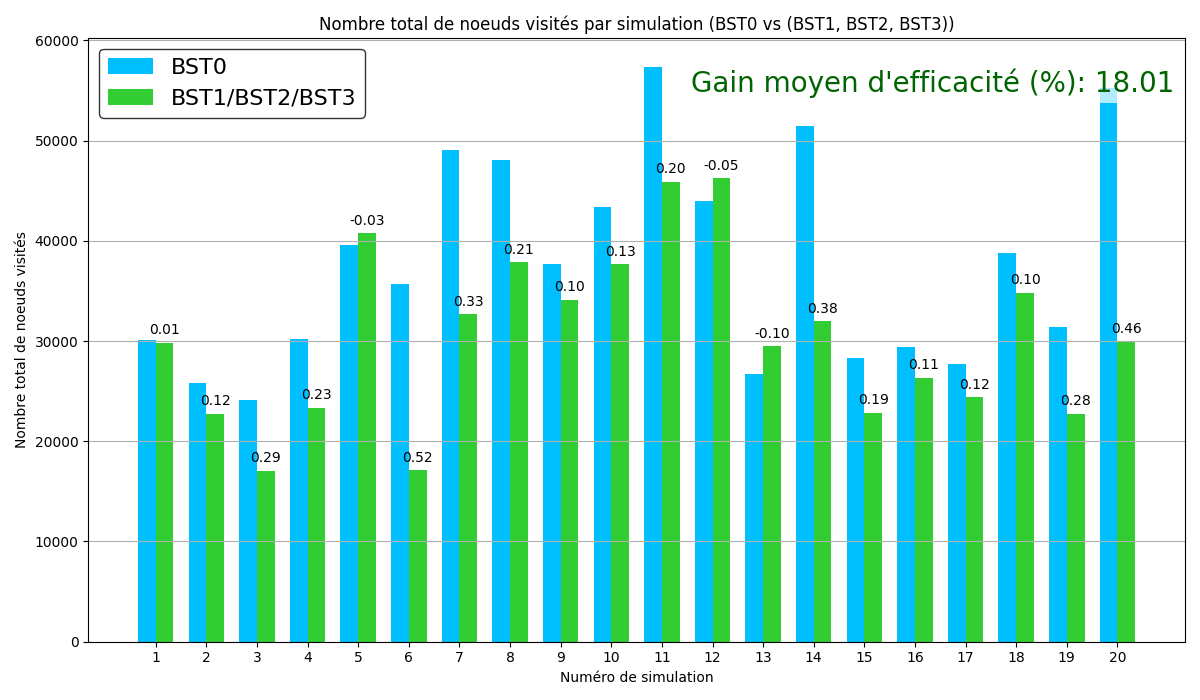
\includegraphics[width=\linewidth, scale=0.5]{rgs}
\end{minipage}
\begin{minipage}{0.4\textwidth}
\small
Le diagramme en barres représente le nombre total de nœuds traversés $\mathbf{T}$ par simulation de recherche par intervalle de mots dans \textbf{BST0} et le triplet \textbf{(BST1, BST2, BST3)}. L'intervalle $\left[\mathit{Mot}_1,\ \mathit{Mot}_2\right]$ est choisi aléatoirement avec $(\mathit{Mot}_1, \mathit{Mot}_2) \in \mathit{E} \times \mathit{E}$, où $\mathit{E}$ désigne l'ensemble des mots extraits d'un fichier $\mathit{F}$ comportant $N \geq 10000$ mots générés aléatoirement. Sur un total de $n = 20$ simulations, les arbres restructurés montrent un gain moyen d'efficacité de \[\Delta = \frac{1}{n} \sum_{i=1}^{n} \frac{T_{BST0_i} - T_{trip_i}}{T_{BST0_i}} \times 100\% \approx \mathbf{18{,}01\%}.\]
\end{minipage}
\end{figure}

\subsection{Conclusion}
\small
Les résultats confirment que la structure de l’arbre a une influence déterminante sur l’efficacité des recherches par intervalle. Les arbres réorganisés \textbf{(BST1, BST2, BST3)} permettent une traversée plus optimisée par rapport à \textbf{BST0}.

\section{Recherche d'un mot singulier}

\begin{figure}[h]
\centering
\begin{minipage}{0.30\textwidth}
	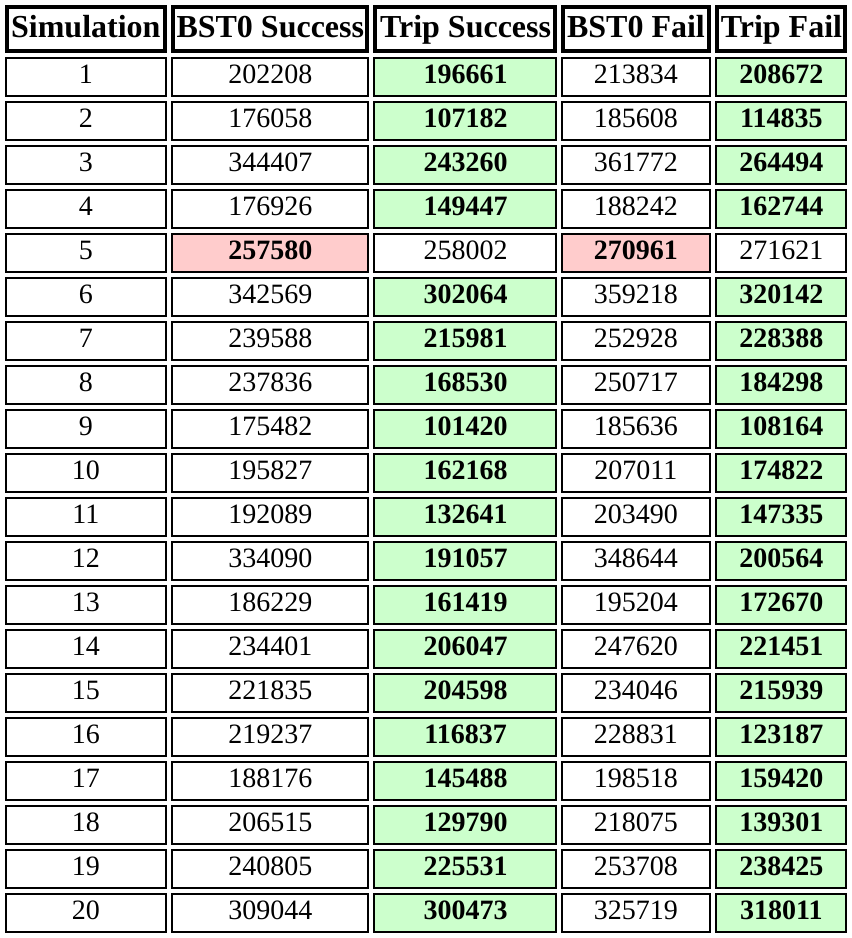
\includegraphics[width=\linewidth, scale=0.05]{tsws}
\end{minipage}
\begin{minipage}{0.60\textwidth}
	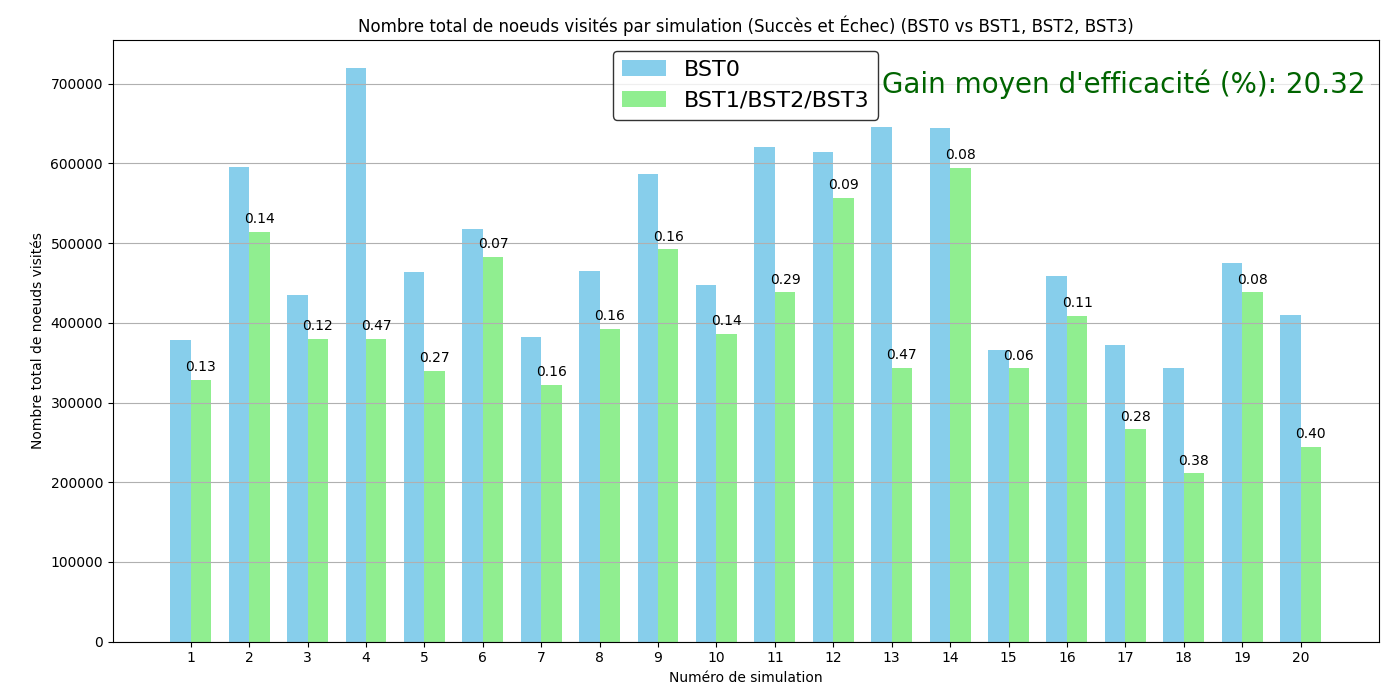
\includegraphics[width=\linewidth, scale=0.5]{sws}
\end{minipage}
\end{figure}

\small
Le tableau détaille, pour chaque simulation, le nombre de nœuds traversés en distinguant les cas de succès et d’échec pour les arbres \textbf{BST0} et \textbf{(BST1, BST2, BST3)}. Le diagramme en barres, quant à lui, représente la somme totale des nœuds traversés $\mathbf{T^{\prime}}$  (\textit{Succès + Échec}) pour chacun des deux types d’arbre, afin d’offrir une vision globale de leur performance. Les mots $\mathit{Mot}$ sont choisis aléatoirement, avec $\mathit{Mot} \in \mathit{E}$. Pour $n = 20$ simulations, on observe que le triplet d'arbres montre un gain moyen d'efficacité de $\Delta \approx \mathbf{20{,}32\%}$, en considérant l’ensemble des cas de succès et d’échec.
\subsection{Conclusion}
\small
La simulation met en évidence l’impact de la structure des arbres sur les performances de recherche d'un mot singulier. Le triplet d'arbres réorganisé \textbf{(BST1, BST2, BST3)} permet une exploration plus efficace que l’arbre de référence \textbf{BST0}. 

\section{Conclusion globale}
En résumé, les simulations confirment que la réorganisation des arbres améliore significativement l’efficacité des recherches, aussi bien pour des mots isolés que pour des intervalles, en réduisant le coût moyen de parcours des nœuds.

\vspace{0.3cm}
{\scriptsize \textit{Rachid Mustapha Amine – Groupe 12 \hfill \today}}

\end{document}